
%(BEGIN_QUESTION)
% Copyright 2014, Tony R. Kuphaldt, released under the Creative Commons Attribution License (v 1.0)
% This means you may do almost anything with this work of mine, so long as you give me proper credit

This cross-limited air/fuel ratio control system is supposed to maintain the fuel-to-air ratio at 1:1 for all firing conditions.  Suppose it has been functioning properly for a long time at a 30\% firing rate (i.e. firing command signal = 30\%; air flow = 30\%; fuel flow = 30\%):

$$\includegraphics[width=15.5cm]{i00932x01.eps}$$

\noindent
Choose the best answer describing the immediate effect on this process if the air flow transmitter suddenly fails with a {\it high} signal:

\begin{itemize}
\item{} The burner's fuel/air mixture will become {\it rich} (i.e. too much fuel for the amount of air)
\vskip 10pt
\item{} The burner's fuel/air mixture will become {\it lean} (i.e. too much air for the amount of fuel)
\vskip 10pt
\item{} Both air and fuel valves will shut off causing the burner to go out
\vskip 10pt
\item{} Both air and fuel valves will open 100\% causing the burner to output maximum fire
\end{itemize}

\underbar{file i00932}
%(END_QUESTION)





%(BEGIN_ANSWER)

The burner's fuel/air mixture will become {\it rich} (i.e. too much fuel for the amount of air)

%(END_ANSWER)





%(BEGIN_NOTES)

{\bf This question is intended for exams only and not worksheets!}.

%(END_NOTES)


